\documentclass[conference]{IEEEtran}

\usepackage{graphicx}\graphicspath{{figs/}}
\usepackage{color}
\usepackage{amsmath}
\usepackage{amsfonts}
\usepackage{amssymb}
\usepackage{amsthm}
\usepackage{multicol}
\usepackage{multirow}
\usepackage{xspace}
\usepackage{listings}
\usepackage{ifthen}
\usepackage{float} % defines newfloat used below
%\usepackage[sort&compress]{natbib} % <<<<<<<<<<<<<<<<<<<<<<<<<<<<<<<<<<<< commented out
%\usepackage{todos} % Use \todoset{all=off} to turn off todos in a paper.
\usepackage{booktabs}
\usepackage{fancyhdr}
\usepackage{microtype}
\usepackage{paralist}

% hyperref redefines a number of macros, so it should be last.  Empirically,
% doing so eliminates compiler warnings.
\usepackage[bookmarks, colorlinks, citecolor=green, urlcolor=blue,
			filecolor=blue, linkcolor=blue]{hyperref}
% According to the hyperref readme, algorithm must follow hyperref

%~~~~~~~~~~~~~~~~~~~~~~~~~~~~~~~~~~~~~~~~~~~~~~~~~~~~~~~~~~~~~~~~~~~~~~~~~~~~~~
% Macros

% English
\newcommand{\cf}{\hbox{\emph{cf.}}\xspace}
\newcommand{\deletia}{\ldots [deletia] \ldots}
\newcommand{\etal}{\hbox{\emph{et al.}}\xspace}
\newcommand{\eg}{\hbox{\emph{e.g.},}\xspace}
\newcommand{\ie}{\hbox{\emph{i.e.},}\xspace}
\newcommand{\scil}{\hbox{\emph{sc.}}\xspace} %scilicet: it is permitted to know
\newcommand{\st}{\hbox{\emph{s.t.}}\xspace}
\newcommand{\wrt}{\hbox{\emph{w.r.t.}}\xspace}
\newcommand{\etc}{\hbox{\emph{etc.}}\xspace}
\newcommand{\viz}{\hbox{\emph{viz.}}\xspace} %videlicet: it is permitted to see
\newcommand{\vs}{\hbox{\emph{vs.}}\xspace}

\newcommand{\cat}[1]{{\textsc{#1}}}

\usepackage{paralist}
\usepackage{mathrsfs}
\usepackage{tabularx}
\usepackage{subfigure}

\newcommand{\ab}[1]{\todo[Alberto]{#1}}
\newcommand{\cb}[1]{\todo[Chris]{#1}}

\renewcommand{\quotation}[1]{``\emph{#1}''}


\iffalse{
\def\todo#1{{\sf $\natural$ #1 $\natural$}}
\def\note#1{{\sf $\clubsuit$ #1 $\clubsuit$}}
\def\marknote#1{{\sf $\spadesuit$ #1 $\spadesuit$}}
}\fi

%\usepackage{mdframed} <<<<<<<<<<<<<<<<<<<<<<<<<<<<<<<<<<<<<<< commented out
%% Document-specific hyperref options
\hypersetup{
pdftitle={Expectations, Outcomes, and Challenges of Modern Code Review},
    pdfauthor={Alberto Bacchelli and Christian Bird},
    plainpages=false,
    linkcolor=black, % Overriding these colors to black is somewhat unfortunate 
    %citecolor=black, % b/c the defaults are useful in color.
    citecolor=blue, % b/c the defaults are useful in color.
    filecolor=black,
    urlcolor=black,
    pdfpagelabels
}

%% sig-alternative is stupid
%\pdfpagewidth=8.5in
%\pdfpageheight=11in

% for our nicer-looking \paragraphs under sig-alternate
\newlength{\emstr}
\setlength{\emstr}{0.75em plus 1ex minus 1ex}
\newcommand{\boldpara}[1]{%
\vspace{1.5mm}%
\par\noindent\textbf{#1}\hspace{\emstr}
}% 

\newcommand{\figref}[1]{Figure~\ref{#1}\xspace}

\newcounter{copyrightbox}

\title{Expectations, Outcomes, and Challenges \\ 
of Modern Code Review}

\author{
	\begin{tabular}{ccc}
		Alberto Bacchelli & \hspace{0.5in} & Christian Bird \\
		REVEAL @ Faculty of Informatics & & Microsoft Research \\
		University of Lugano, Switzerland & & Redmond, Washington, USA \\
		\texttt{alberto.bacchelli@usi.ch} &  &\texttt{cbird@microsoft.com}
	\end{tabular}
}


%\iffalse{
% Only for camera ready -- prevent TeX from rendering widows
%\widowpenalty=9999
%\clubpenalty=9999 
%}\fi

\begin{document}

\maketitle

\begin{abstract}

Code review is a common software engineering practice employed both in open
source and industrial contexts.  Review today is less formal and more
``lightweight'' than the code inspections performed and studied in the 70s and
80s. We empirically explore the motivations, challenges, and outcomes of
tool-based code reviews. We observed, interviewed, and surveyed developers and
managers and manually classified hundreds of review comments across diverse
teams at Microsoft. Our study reveals that while finding defects remains the
main motivation for review, reviews are less about defects than expected and
instead provide additional benefits such as knowledge transfer, increased team
awareness, and creation of alternative solutions to problems. Moreover, we find
that code and change understanding is the key aspect of code reviewing and that
developers employ a wide range of mechanisms to meet their understanding needs,
most of which are not met by current tools. We provide recommendations for
practitioners and researchers.

\end{abstract}

%\listoftodos

%!TEX root = paper.tex

%%%%%%%%%%%%%%%%%%%%%%
\section{Introduction} \label{sec:introduction}
%%%%%%%%%%%%%%%%%%%%%%


Peer code review, a manual inspection of source code by developers other than
the author, is recognized as a valuable tool for reducing software defects and
improving the quality of software projects (Ackerman, Fowler and Ebenau 1984)
(Ackerman, Buchwald and Lewski 1989). In 1976, Fagan formalized a highly
structured process for code reviewing (Fagan 1976), based on line-by-line group
reviews, done in extended meetings -- code inspections. Over the years,
researchers provided evidence on code inspectionís benefits, especially in
terms of defect finding, but the cumbersome, time-consuming, and synchronous
nature of this approach hinders its universal adoption in practice (Shull
2008).

Nowadays, many organizations are adopting more lightweight code review
practices to limit the inefficiencies of inspections. In particular, there is a
clear trend toward the usage of tools specifically developed to support code
review (Rigby, Cleary, et al. 2012). In the context of this paper, we define
Modern Code Review, as review that is (1) informal (in contrast to
Fagan-style), (2) tool-based, and that (3) occurs regularly in practice
nowadays, for example at companies such as Microsoft, Google (Kennedy 2006),
Facebook (Tsotsis 2011), and in other companies and OSS projects (Gerrit
(software) 2012).

This trend raises questions, such as: Can we apply the lessons learned from
previous research on code inspections to modern code reviews? What are the
expectations for code review nowadays? What are the actual outcomes of code
review? What challenges do people face in code review?

Answers to these questions can provide insight for both practitioners and
researchers.  Developers and other software project stakeholders can use
empirical evidence about expectations and outcomes to make informed decisions
about when to use code review and how it should fit into their development
process. Researchers can focus their attention on practitionersí challenges to
make code review more effective.

We present an in-depth study of practices in teams that use modern code review,
revealing what practitioners think, do, and achieve when it comes to modern
code review.

Since Microsoft is made up of many different teams working on very diverse
products, it gives the opportunity to study teams performing code review in
situ and understand their expectations, the benefits they derive from code
review, the needs they have, and the problems they face.

We set up our study as an explorative investigation. We started without a
priori hypotheses regarding how and why code review should be performed, with
the aim of discovering what developers and managers expect from code review,
how reviews are conducted in practice, and what the actual outcomes and
challenges are. To that end, we (1) observed 17 industrial developers
performing code review with various degrees of experience and seniority across
16 separate product teams with distinct reviewing cultures and policies; (2)
interviewed these developers using a semi-structured interviews; (3) manually
inspected and classified the content of 570 comments in discussions contained
within code reviews; and (4) surveyed 165 managers and 873 programmers.

Our results show that, although the top motivation driving code reviews is
still finding defects, the practice and the actual outcomes are less about
finding errors than expected: Defect related comments comprise a small
proportion and mainly cover small logical low-level issues. At the same time,
code review additionally provides a wide spectrum of benefits to software
teams, such as knowledge transfer, team awareness, and improved solutions to
problems. Moreover, we found that context and change understanding is the key
of any review. According to the outcomes they want to achieve, developers
employ many mechanisms to fulfill their understanding needs, most of which are
not currently met by any code review tool.

This paper makes the following contributions:
\begin{itemize}
  \item Characterizing the motivations of developers and managers for code review and compare with actual outcomes.
  \item Relating the outcomes to understanding needs and discuss how developers achieve such needs.
\end{itemize}

Based on our findings, we provide recommendations for practitioners and
implications for researchers as well as outline future avenues for research.
%!TEX root = ../paper.tex

%%%%%%%%%%%%%%%%%%%%%%
\section{Related Work} \label{sec:related_work}
%%%%%%%%%%%%%%%%%%%%%%


Previous studies have examined the practices of code inspection and
code review.  Stein \etal conducted a study focusing specifically on
distributed, asynchronous code inspections~\cite{stein1997casestudy}. The study included evaluation
of a tool that allowed for identification and sharing of code faults or
defects. Participants at separated locations can then discuss faults via the
tool. Laitenburger conducted a survey of code inspection methods, and presented
a taxonomy of code inspection techniques~\cite{laitenberger2002survey}. Johnson conducted
an investigation into code review practices in OSS development and their
effect on choices made by software project managers~\cite{johnson2006collaboration}.

Porter \etal~\cite{porter1996review} reported on a review of studies on
code inspection in 1995 that examined the effects of factors such as team size,
type of review, and number of sessions on code inspections.  They also assessed
costs and benefits across a number of studies.  These studies differ from ours
in that they were not tool-based and were the majority involved planned
meetings to discuss the code.

However, prior research also sheds light on why review today is more often
tool-based, informal, and often asynchronous. The current state of code review
might be due to the time required for more formal inspections.  Votta found
that 20\% of the interval in a ``traditional inspection'' is wasted due to
scheduling~\cite{votta1993does}. The ICICLE tool~\cite{brothers1990icicle}, or ``Intelligent Code Inspection in a C Language Environment,'' was
developed after researchers at Bellcore observed how much time and work was
expended before and during formal code inspections. Many of todayís review
tools are based on ideas that originated in ICICLE.  Other similar tools have
been developed in an effort to reduce time for inspection and allow
asynchronous work on reviews.   Examples include CAIS~\cite{mashayekhi1994cais} 
and Scrutiny~\cite{gintell1993scrutiny}.

More recently, Rigby has done extensive work examining code review practices in
OSS development~\cite{rigby2008open, Rigb2011a, rigby2012open}.  For example in
a study of practices in the Apache project~\cite{rigby2008open},
they data-mined the email archives and found that reviews were typically small
and frequent, and that the contributions to a review were often brief and
independent from one another.

Sutherland and Venolia conducted a study at Microsoft regarding using code
review data for later information needs~\cite{sutherland2009can}. They
hypothesized that the knowledge exchanged during code reviews could be of great
value to engineers later trying to understand or modify the discussed code.
They found that \quotation{the meat of the code review dialog, no matter what medium, is
the articulation of design rationale} and, thus, \quotation{code reviews are an enticing
opportunity for capturing design rationale.}

When studying developer work habits, Latoza \etal found that many problems
encountered by developers were related to understanding the rationale behind
code changes and gathering knowledge from other members of their team~\cite{latoza2006maintaining}.
%!TEX root = ../paper.tex

%%%%%%%%%%%%%%%%%%%%%%
\section{Methodology} \label{sec:methodology}
%%%%%%%%%%%%%%%%%%%%%%


In this section we define the research questions, describe the research
settings, and outline our research method.

\subsection{Research Questions}

Our investigation of code review revolves around the following research
questions, which we iteratively refined during our initial in-field
observations and interviews:

\begin{enumerate}
  \item What are the motivations and expectations for modern code review? Do they change from managers to developers and testers?
  \item What are the actual outcomes of modern code review? Do they match the expectations?
  \item What are the main challenges experienced when performing modern code reviews relative to the expectations and outcomes?
\end{enumerate}

\subsection{Research Setting}

Our study took place with professional developers, testers, and managers.
Microsoft develops software in diverse domains, from high end server enterprise
data management solutions such as SQL Server to mobile phone applications and
smart phone apps to search engines. Each team has its own development culture
and code review policies. Over the past two years, a common tool for code
review at Microsoft has achieved wide-spread adoption. As it represents a
common and growing solution for code review (over 40,000 developers used it so
far), we focused on developers using this tool for code review---\emph{CodeFlow}. 

CodeFlow is a collaborative code review tool that allows users to directly
annotate source code in its viewer and interact with review participants in a
live chat model. The functionality of CodeFlow is similar to other review tools
such Google's Mondrian~\cite{kennedy2006online}, Facebook's Phabricator~\cite{tsotsis2011online} or
open-source Gerrit~\cite{gerrit2012online}. Developers who want their code to
be reviewed create a package with the changed (new, deleted, and modified)
files, select the reviewers, write a message to describe the code review, and
submit everything to the CodeFlow service. CodeFlow then notifies the reviewers
about the incoming task via email.



Once reviewers open a CodeFlow review, they interact with it via a single
desktop window (\figref{fig:codeflow:screenshot}). On the top left (\textbf{1}), they see the list of files
changed in the current submission, plus a ``description.txt'' file, which
contains a textual explanation of the change, written by the author. On bottom
left, CodeFlow shows the list of reviewers and their status (\textbf{2}). We see that
Christian is the review author and Alberto, Tom, and Nachi are the reviewers.
Alberto has reviewed and is waiting for the author to act, as the clock icon
suggests, while Nachi already signed off on the changes. CodeFlow's main view
(\textbf{3}) shows the diff-highlighted content of the file currently under review. Both
the reviewers and the author can highlight portions of the code and add
comments inline (\textbf{4}). These comments can start threads of discussion and are the
interaction points for the people involved in the review. Each user viewing the
same review in CodeFlow sees events as they happen.  Thus, if an author and
reviewer are working on the review at the same time, the communication is
synchronous and comment threads act similar to instant messaging. The comments
are persisted so that if they work at different times, the communication
becomes asynchronous. The bottom right pane (\textbf{5}) shows the summary of all the
comments in the review. 

CodeFlow centralizes and records all the information on code reviews on a
central server. This provides an additional data source that we used to analyze
real code review comments without incurring the Hawthorne effect~\cite{adair1984hawthorne}.



\begin{figure}[t] %  figure placement: here, top, bottom, or page
   \centering
   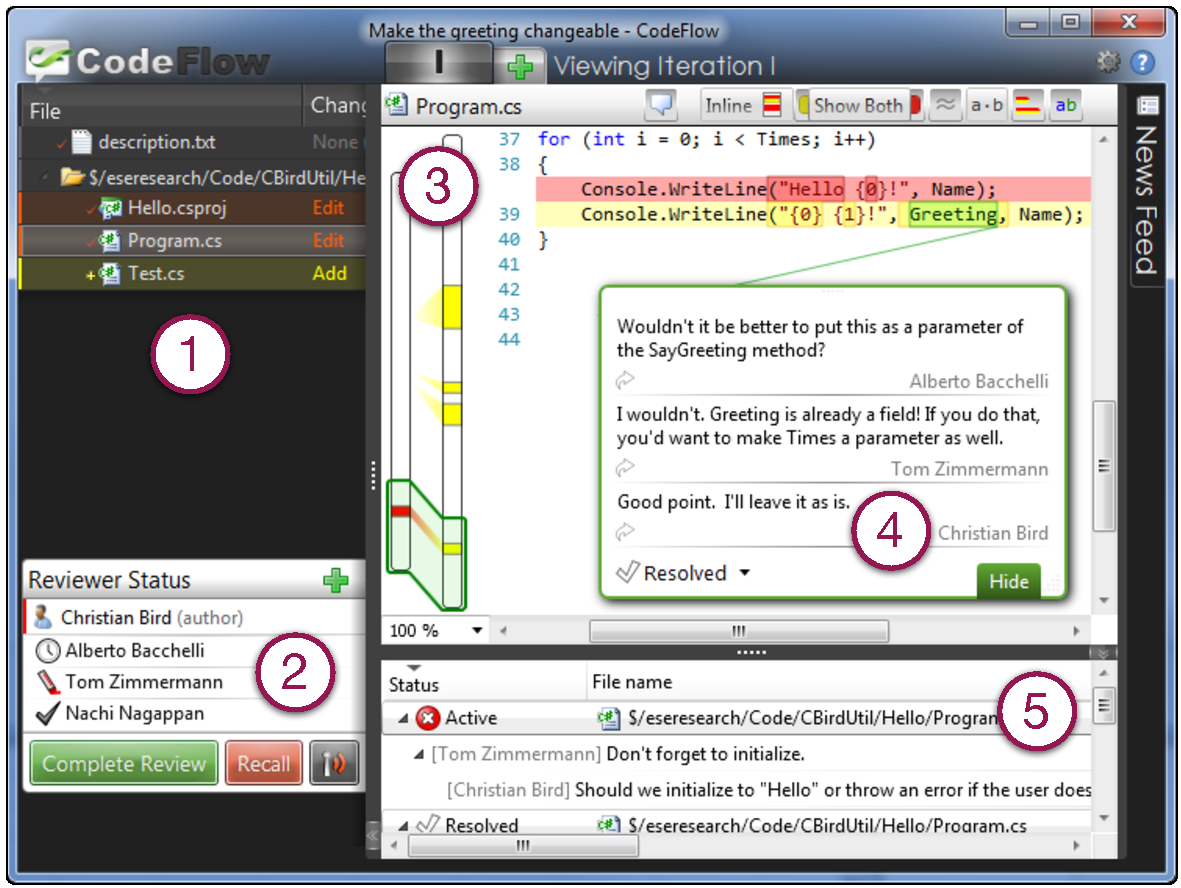
\includegraphics[width=0.98\columnwidth]{codeflow.pdf}
   \caption{CodeFlow, the main code review tool used by developers at Microsoft.}
   \label{fig:codeflow:screenshot}
      \vspace{-1.5em}
\end{figure}



\subsection{Research Method}

\begin{figure*}[t] %  figure placement: here, top, bottom, or page
   \centering
   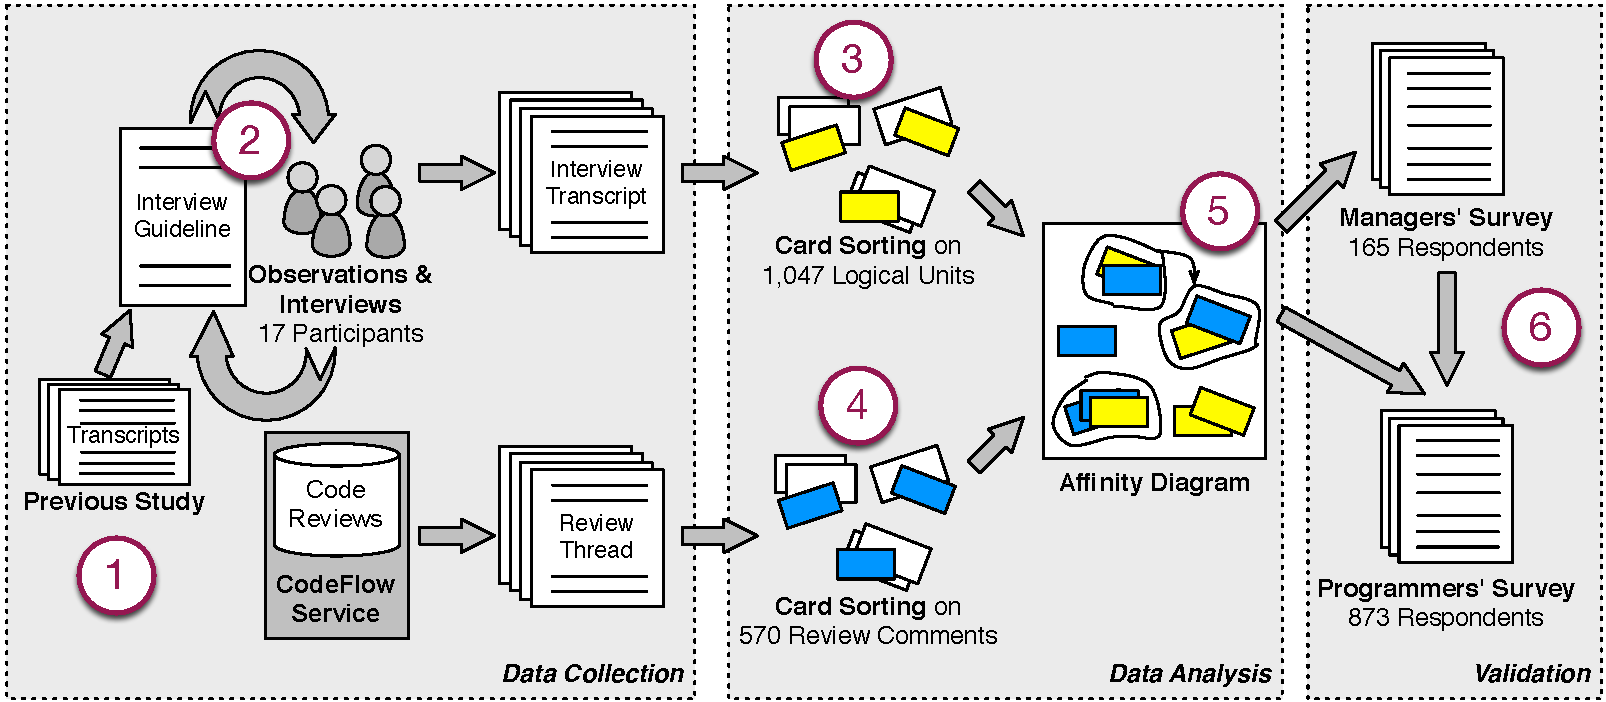
\includegraphics[width=1.4\columnwidth]{methodology.pdf}
   \caption{The mixed approach research method applied.}
   \label{fig:research-method}
   \vspace{-1.5em}
\end{figure*}

Our research method followed a mixed approach~\cite{creswell2009research}, depicted in
\figref{fig:research-method}, collecting data from different sources for triangulation: (\textbf{1})
analysis of previous study, (\textbf{2}) observations and interviews with developers,
(\textbf{3}) card sort on interview data,  (\textbf{4}) card sort on code review comments, (\textbf{5})
the creation of an affinity diagram, and (\textbf{6}) survey to managers and
programmers.

\textbf{1. Analysis of previous study:} Our research started with the analysis of a
study commissioned by Microsoft, between April and May 2012 carried out by an
external vendor. The study investigated how different product teams were using
CodeFlow. It consisted of structured interviews (lasting 30-50 minutes) to 23
people with different roles.

Most of the interview questions revolved around topics that are very specific
to tool usage, and were only tangentially related to this work. We found one
relevant as a starting point for our study: ``\emph{What do you hope to accomplish
when you submit a code review?}'' We analyzed the transcript of this answer, for
each interview, through the process of \emph{coding}~\cite{berg2004qualitative} (also used in
\emph{grounded theory}~\cite{adolph2011using}): breaking up the answers into smaller coherent
units (sentences or paragraphs) and adding \emph{codes} to them. We organized codes
into \emph{concepts}, which in turn were grouped into more abstract \emph{categories}.

From this analysis, four motivations emerged for code review: finding defects,
maintaining team awareness, improving code quality, and assessing the
high-level design. We used them to draw an initial guideline for our
interviews.

\textbf{2. Observations and interviews with developers:} Next, we conducted a series of
one-to-one meetings with developers who use CodeFlow, each taking 40-60
minutes. 

We contacted 100 randomly selected candidates who signed-off between 50 and 250 code
reviews since the CodeFlow release and sampled across different product teams
to address our research questions from a \emph{multi-point} perspective. We wrote
developers who used CodeFlow in the past and asked them to contact us, giving
us 30 minute notice when they received their next review task so that we could
observe.  The respondents that we interviewed comprised five developers, four
senior developers, six testers, one senior tester, and one software architect.
Their time in the company ranged from 18 months to almost 10 years, with a
median of five years. 

Each meeting was comprised of two parts: In the first part, we observed them
performing the code review that they had been assigned. To minimize
invasiveness we used only one observer and to encourage the participant to
narrate their work, we asked the participants to think of us as a newcomer to
the team. In this way, most developers thought aloud without need of prompting.
With consent, we recorded the audio, assuring the participants of anonymity.
Since we, as observers, have backgrounds in software development and practices
at Microsoft, we were able to understand most of the work and where and how
information was obtained without inquiry. 

The second part of the meeting was a \emph{semi-structured} interview~\cite{taylor2010qualitative}. Semi-structured interviews make use of an \emph{interview guide} that
contains general groupings of topics and questions rather than a pre-determined
exact set and order of questions.  They are often used in an exploratory
context to ``find out what is happening [and] to seek new insights''~\cite{weiss1995learning}. 
The guideline was iteratively refined after each interview, in
particular when developers started providing answers very similar to the
earlier ones, thus reaching a saturation effect.

Observations also reached a \emph{saturation} point, thus providing insights very similar to the earlier ones. For this, after the first 5-6 observations, we adjusted the meetings to have shorter observations, which we used as a starting point for our meetings and as a ``hook'' to talk about topics in our guideline.

The audio of each interview was then transcribed and broken up into smaller
coherent units for subsequent analysis.

\textbf{3. Card sort (meetings):} To group codes that emerged from interviews and
observations into categories, we conducted a \emph{card sort}. Card sorting is a
sorting technique that is widely used in information architecture to create
mental models and derive taxonomies from input data~\cite{barker2005online}. In our case
it helped to organize the codes into hierarchies to deduce a higher level of
abstraction and identify common themes. A card sort involves three phases: In
the \begin{inparaenum}[(1)]
\item \emph{preparation phase}, participants of the card sort are selected and the
cards are created; in the 
\item \emph{execution phase}, cards are sorted into meaningful
groups with a descriptive title; and in the 
\item \emph{analysis phase}, abstract hierarchies are formed to deduce general categories.
\end{inparaenum}

We applied an \emph{open card sort}: There were no predefined groups. Instead, the
groups emerged and evolved during the sorting process. In contrast, a closed
card sort has predefined groups and is typically applied when themes are known
in advance, which was not the case for our study.

The first author of this paper created all of the cards, from the 1,047
coherent units in the interviews. Throughout our further analysis other
researchers (the second author and external people) were involved in developing
categories and assigning cards to categories, so as to strengthen the validity
of the result. The first author played a special role of ensuring that the
context of each question was appropriately considered in the categorization,
and creating the initial categories. To ensure the integrity of our categories,
the cards were sorted by the first author several times to identify initial
themes. Next, all researchers reviewed and agreed on the final set of
categories.

\textbf{4. Card sort (code review comments):} The same method was applied to group code
review comments into categories: We randomly sampled 200 threads with at least
two comments (e.g., Point 4 of \figref{fig:research-method}), from the entire dataset of CodeFlow
reviews, which embeds data from dozens of independent software products at
Microsoft. We printed one card for each comment (along with the entire
discussion thread to give the context), totaling 570 cards, and conducted a
card sort, as performed for the interviews, to identify common themes.

\textbf{5. Affinity Diagram:} We used an \emph{affinity diagram} to organize the categories
that emerged from the card sort. This tool allows large numbers of ideas to be
sorted into groups for review and analysis~\cite{shade2000improving}. We used it
to generate an overview of the topics that emerged from the card sort, in order
to connect the related concepts and derive the main themes. For generating the
affinity diagram, we followed the five canonical steps: we \begin{inparaenum}[(1)] 
\item recorded the categories on post-it-notes, 
\item spread them onto a wall, 
\item sorted the categories based on discussions, until all are sorted and all participants agreed, 
\item named each group, and 
\item captured and discussed the themes.
\end{inparaenum}


\textbf{6. Surveys:} The final step of our study was aimed at validating the
concepts that emerged from the previous phases. Towards this goal, we created
two surveys to reach a significant number of participants and to challenge our
conclusions (The full surveys are available as a technical report~\cite{bacchelli2012appendix}). 
For the design of the surveys, we followed Kitchenham and
Pfleeger's guidelines for personal opinion surveys~\cite{kitchenham2008personal}. 
Both surveys were anonymous to increase response rates~\cite{tyagi1989effects}.

We sent the first survey to a cross section of managers.  We considered
managers for which at least half of their team performed code reviews regularly
(on average, one per week or more) and sampled along two dimensions.  The first
dimension was whether or not the manager had participated in a code review
himself since the beginning of the year and the second dimension was whether
the manager managed a single team or multiple teams (a manager of managers).
Thus, we had one sample of first level managers who participated in review,
another sample of second level managers who participated in reviews, \etc  The
first survey was a short survey comprising 6 questions (all optional), which we
sent to 600 managers that had at least 10 direct or indirect reporting
developers who used CodeFlow. The central focus was the open
question asking to enumerate the main motivations for doing code reviews in
their team. We received 165 answers (28\% response rate), which we analyzed
before devising the second survey.

The second survey comprised 18 questions, mostly closed with multiple choice
answers, and was sent to 2,000 randomly chosen developers who signed off on
average at least one code review per week since the beginning of the year. We
used the time frame of January to June of 2012 to minimize the amount of
organizational churn during the time period and identify employees' activity in
their current role and team.  We received 873 answers (44\% response rate). Both
response rates were  high, as other online surveys in software engineering have
reported response rates ranging from 14\% to 20\%~\cite{punter2003conducting}.





%!TEX root = paper.tex

%%%%%%%%%%%%%%%%%%%%%%
\section{Why Do Programmers Do Code Reviews} \label{sec:expectations}
%%%%%%%%%%%%%%%%%%%%%%


Our first research question seeks to understand what motivations and
expectations drive code reviews, and whether managers and developers share the
same opinions.

Based on the responses that we coded from observations of developers performing
code review as well as interviews, there are various motivations for code
review. Overall, the interviews revealed that finding defects, even though
prominent, is just one of the many motivations driving developers to perform
code reviews. Especially when reinforced by a strong team culture around
reviews, developers see code reviews as an activity that has multiple
beneficial influences not only on the code, but also for the team and the
entire development process. In this vein, one senior developerís comment
summarized many of the responses: \quotation{[code review] also has several
beneficial influences: (1) makes people less protective about their code, (2)
gives another person insight into the code, so there is (3) better sharing of
information across the team, (4) helps support coding conventions on the team,
and [...] (5) helps improving the overall process and quality of code.}

Through the card sort on both meetings and code review comments, we found
several references to motivations for code review and identified six main
topics. To complete this list, in the survey for managers, we included an open
question on why they perform code reviews in their team. We analyzed the
responses to create a comprehensive list of high-level motivations. We included
this list in the developersí survey and asked them to rank the top three main
reasons that described why they do code reviews.

In the rest of this section, we discuss the motivations that emerged as the
most prominent. We order them according to the importance they were given by
the 873 developers and testers who responded to the final survey.

\subsection{Finding Defects}

One interviewed senior tester explains that he performs code reviews because
they \quotation{are a great source of bugs;} he goes even further stating:
\quotation{sometimes code reviews are a cheaper form of bug finding than
testing.} Moreover, the tool seems not to have an impact on this main
motivation: \quotation{using CodeFlow or using any other tool makes a little
difference to us; it's more about being able to identify flaws in the logic.}

Almost all the managers included ``finding defects'' as one of the reasons for
doing code reviews; for 44\% of the managers, it is the top reason. Managers
considered defects to be both low level issues (e.g., \quotation{correct logic
is in place}) and high level concerns (e.g., \quotation{catch errors in
design}). Concerning surveyed developers/testers, ``finding defects'' is the
first motivation for code review for 383 of the programmers (44\%), second
motivation for 204 (23\%), and third for 96 (11\%).

This is in-line with the reason why code inspections were devised in the first
place: reducing software defects (Ackerman, Fowler and Ebenau 1984).

Nevertheless, even though ``finding defects'' emerged from our data as a strong
motivation (the first for almost half of the programmers and managers),
interviews and survey results indicate that this only tells part of the story
of why practitioners do code reviews and the outcomes they expect.

\subsection{Code Improvement}

Code improvements are comments or changes about code in terms of readability,
commenting, consistency, dead code removal, etc., but do not involve
correctness or defects.

Programmers ranked ``code improvement'' as an important motivation for code
review, close to ``finding defects:'' This is the primary motivation for 337
programmers (39\%), the second for 208 (24\%), and the third for 135 (15\%).
Managers reported code improvements as their primary motivation in 51 cases
(31\%). One manager wrote how code review in her view is a
\quotation{discipline of explaining your code to your peers [that] drives a
higher standard of coding. I think the process is even more important than the
result.}

Most interviewed programmers mentioned that at least one of the reviewers
involved in each code review takes care of checking whether the code follows
the team conventions, for example in terms of code formatting and in terms of
function and variable naming. Some programmers use the ``code improvement''
check as a first step when doing code review: \quotation{the first basic pass
on the code is to check whether it is standard across the team.}

The interviews also gave us a glimpse of the connection between the quality of
code reviews and ``code improvement'' comments. Such comments seem easier to
write and sometimes interviewees mentioned them as the way reviewers use to
avoid spending time to conduct good code reviews. An observation by a senior
developer, in the company for more than nine years, summarizes the opinions we
received from many interviewees: \quotation{Iíve seen quite a few code reviews
where someone commented on formatting while missing the fact that there were
security issues or data model issues.}

\subsection{Alternative Solutions}

``Alternative solutions'' regard changes and comments on improving the
submitted code by adopting an idea that leads to a better implementation. This
is one of the few motivations in which developers and managers do not agree.
While 147 (17\%) developers put this as the first motivation, 202 (23\%) as the
second, and 152 (17\%) as the third, only 4 managers (2\%) even mentioned it
(e.g., \quotation{Generate better ideas, alternative approaches} and
\quotation{Collective wisdom: Someone else on the project may have a better
idea to solve a problem}). The outcome of the interviews was similar to the
position of managers: Interviewees vaguely mentioned this motivation, and
mostly in terms of generic \quotation{better ways to do things.}


\subsection{Knowledge Transfer}

All the interviewees but one motivated their code reviews also from a learning,
or ``knowledge transfer,'' perspective. With the words of a senior developer:
\quotation{one of the things that should be happening with code reviews over
time is a distribution of knowledge. If you do a code review and did not learn
anything about the area and you still do not know anything about the area, then
that was not as good code review as it could have been.} Although we did not
include questions related to ``knowledge transfer'' in our interview guideline,
this topic kept emerging spontaneously from each meeting, thus underscoring its
value for practitioners.

Sometimes programmers told us that they follow code reviews explicitly for
learning purposes. For example, a tester explained: \quotation{[I read code
reviews because] from a code review you can learn about the different parts you
have to touch to implement a certain feature.}

According to interviewees, code review is a learning opportunity for both the
author of the change and the reviewers: There is a bidirectional knowledge
transfer about APIs usage, system design, best practices, team conventions,
\quotation{additional code tricks,} etc. Moreover code reviews are recognized
for educating new developers about code writing.

Managers included ``knowledge transfer'' as one of the reasons for code review,
although never as the top motivation. They mostly wrote about code review as an
education means by mentioning among the motivations for code review:
\quotation{developer education,} \quotation{education for junior developers who
are learning the codebase,} and \quotation{learning tool to teach more junior
team members.}

Programmers answering the survey declared ``knowledge transfer'' to be their
first motivation for code review in 73 cases (8\%), their second in 119 (14\%),
and their third in 141 (16\%).

\subsection{Team Awareness and Transparency}

During one of our observations, one developer was preparing a code review
submission as an author: He wanted other developers to \quotation{double check}
his changes before committing them to the repository. After preparing the code,
he specified the developers he wanted to review his code; he required not only
two specific people, but he also put a generic email distribution group as an
\quotation{optional} reviewer. When we inquired about this choice, he explained
us: \quotation{I am adding [this alias], so that everybody [in the team] is
notified about the change I want to do before I check it in.} In the subsequent
interviews, this concept of using an email list as optional reviewer, or
including specific optional reviewers exclusively for awareness emerged again
frequently, e.g., \quotation{Code reviews are good FYIs [for your
information].}

Managers often mentioned the concept of team awareness as a motivation for code
review, frequently justifying it with the notion of ``transparency:'' Not only
must the team be kept aware of the directions taken by the code, but also
nobody should be allowed to ``secretly'' make changes that might break the code
or alter functionalities.

The 873 programmers answering the survey ranked ``team awareness and
transparency'' very close to ``knowledge transfer.'' In fact, the two concepts
appeared logically related also in the interviews; for example one tester,
while reviewing some code said: \quotation{oh, this guy just implemented this
feature, and now let me back and use it somewhere else.} Showing that he both
learned about the new feature and he was now aware of the possibility to use it
in his own code. 75 (9\%) developers considered team awareness their first
motivation for code review, 108 (12\%) their second, and 149 (17\%) their
third. 

Although team awareness and transparency emerged from our data as clearly
promoted by the code review process, academic research seems to have given
little attention to it. 

\subsection{Share Code Ownership}

The concept of ``shared code ownership'' is closely related to ``team awareness
and transparency,'' but it has a stronger connotation toward active
collaboration and overlapping coding activities. Programmers and managers
believe that code review is not only an occasion to notify other team members
about incoming changes, but also a means to have more than one knowledgeable
person about specific parts of the codebase. A manager put the following as her
second motivation for code review: \quotation{Broaden knowledge \& understanding
of how specific features/areas are designed and implemented (e.g., grooming
``backup developers'' for areas where knowledge is too concentrated on one or
two expert developers.}

Moreover, both developers and managers have the opinion that practicing code
review also improves the personal perception of team members about shared code
ownership. On this note, a senior developer, with more than 30 years in the
software industry, explained: \quotation{In the past people did not use to do
code reviews and were very reluctant to put themselves in positions where they
were having other people critiquing their code. The fact that code reviews are
considered as a normal thing helps immensely with making people less protective
about their code.} Similarly a manager wrote us explaining that she deems code
reviews important because they \quotation{Dilute any ``rigid sense of
ownership'' that might develop over chunks of code.}

In the programmersí survey, 51 respondents (6\%) marked ``share code
ownership'' as their first motivation, 100 (11\%) as their second, and (10\%)
as their third.

\subsection{Summary}

In this section, we analyzed the motivations that developers and managers have
for doing code review. We abstracted them into a list, which we finally
included in the programmersí survey. Figure 3 reports the answers given to this
question: The black bar is the number of developers that put that row as their
top motivation, the gray bar is the number that put it as the second
motivation, etc. We have ordered the factors by giving 3 points for a first
motivation response, 2 points for a second motivation, etc. and then sorting by
the sum. 

We discussed the five most prominent motivations, which show that ``finding
defects'' is the top motivation, although participants believe that code review
brings other benefits. The first two motivations were already popular in
research and their effectiveness have been evaluated in the context of code
inspections; on the contrary, the other motivations are still unexplored,
especially those regarding more ``social'' benefits on the team, such as shared
code ownership.

Although motivations are well defined, we still have to verify whether they
actually translate into real outcomes of a modern code review process. 

%!TEX root = paper.tex

%%%%%%%%%%%%%%%%%%%%%%
\section{The Outcomes of Code Reviews} \label{sec:outcomes}
%%%%%%%%%%%%%%%%%%%%%%



%!TEX root = ../paper.tex

%%%%%%%%%%%%%%%%%%%%%%
\section{What Are The Challenges of Code Review?} \label{sec:challenges}
%%%%%%%%%%%%%%%%%%%%%%


Our third research question seeks to understand the main challenges faced by reviewers when performing modern code reviews, also with respect to the expected outcomes. We also seek to uncover the reasons behind the mismatch between expectations and actual outcomes on finding defects in reviews.


\subsection{Code Review is Understanding}

Even though we did not ask any specific question concerning understanding, the theme emerged clearly from our interviews. Many interviewees eventually acknowledged that understanding is their main challenge when doing code reviews. For example, a senior developer autonomously explained to us: \quotation{the most difficult thing when doing a code review is understanding the reason of the change;} a tester, in the same vein: \quotation{the biggest information need in code review: what instigated the change;} and another senior developer: \quotation{in a successful code review submission the author is sure that his peers understand and approve the change.} Although the textual description should help reviewers understanding, some developers do not find it useful: \quotation{people can say they are doing one thing, while they are doing many more of them,} or \quotation{the description is not enough;} in general, developers seem to confirm that \quotation{not knowing files (or {\normalfont [dealing with]} new ones) is a major reason for not understanding a change.}

\begin{figure}[t] %  figure placement: here, top, bottom, or page
   \centering
   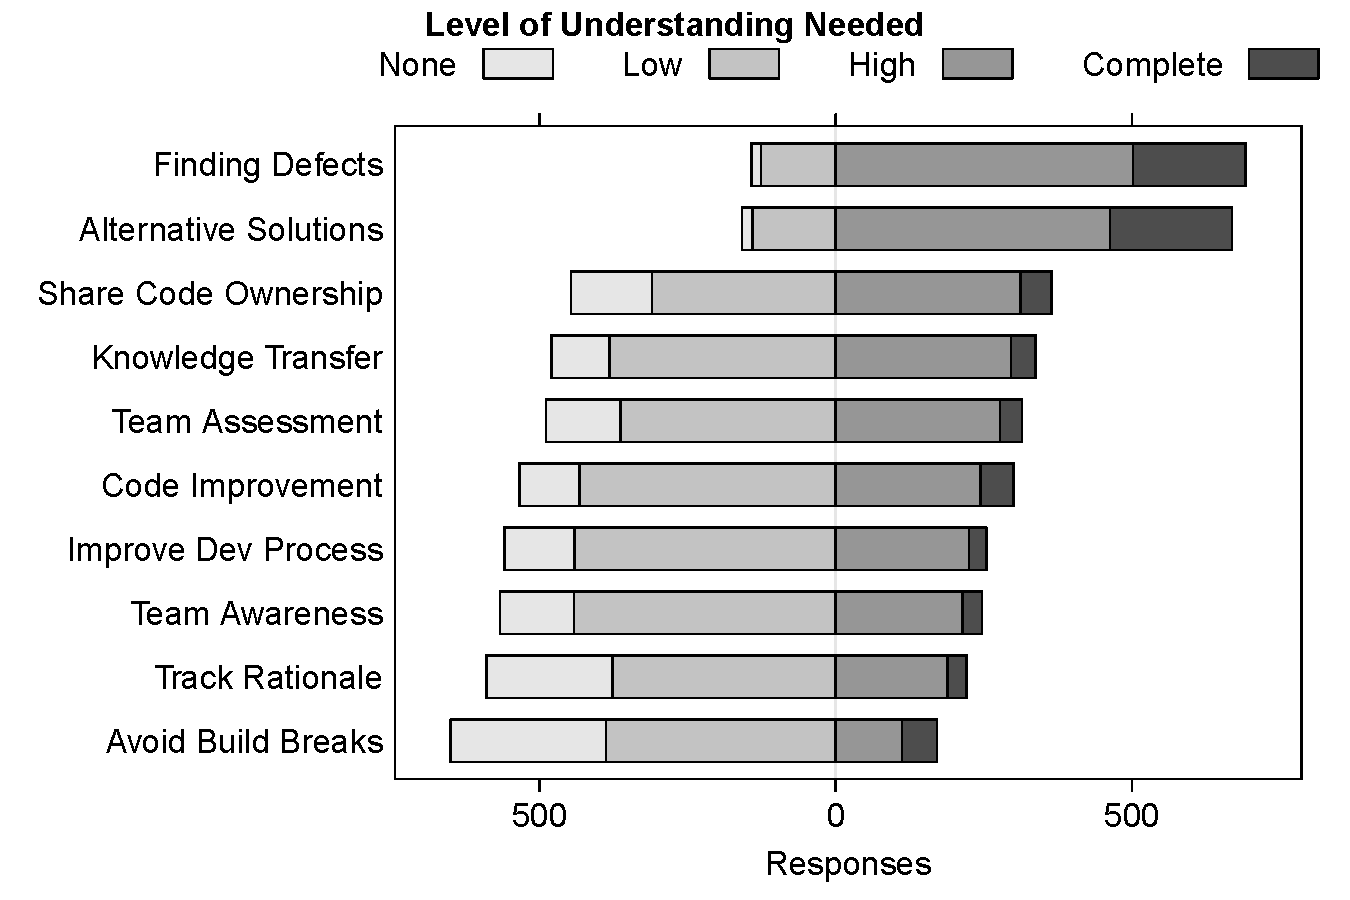
\includegraphics[width=\columnwidth]{understanding.pdf}
   \vspace{-1.5em}
   \caption{Developers' responses in surveys of the amount of code understanding for code review outcomes.}
   \label{fig:understanding}
   \vspace{-1.5em}
\end{figure}

From interviews, no other code review challenge emerged as clearly as understanding the submitted change. Even though scheduling and time issues also appeared challenging, we could always trace them back to the first challenge through the words of a tester: \quotation{understanding the code takes most of the reviewing time.} On the same note, in the code review comments we analyzed, the second most frequent category concerns understanding. This category includes clarification questions and doubts raised by the reviewers who want to grasp the rationale of the changes done on the code, and the corresponding clarification answers. This is also in line with the evidence delivered by Sutherland \& Venolia on the relevance of rationale articulation in reviews~\cite{sutherland2009can}.

Do understanding needs change with the expected outcome of code review? We included a question in the programmers' survey to know how much understanding they needed to achieve each of the motivations listed in \figref{fig:dev-motivations}. The outcome of the question is summarized in \figref{fig:understanding}. The respondents could answer with a four values Likert's scale, by selecting the understanding of the change they felt was required to achieve the specific outcome. The most difficult task from the understanding perspective is \emph{finding defects}, immediately followed by \emph{alternative solutions}. Both clearly stand out from the other items. The gap in understanding needs between \emph{finding defects} and \emph{code improvement} seems to corroborate our hypothesis that the difference in the number of comments about these two items in review comments is mostly due to understanding issues. Thus, if managers and developers want code review to match their need for \emph{finding defects}, context and change understanding must be improved.


\subsection{Code Review is Understanding}

By observing developers performing code reviews, we noticed that some started code reviews by thoroughly reading the accompanying textual description, while others went directly to a specific changed file. In the first group, the time required for putting the first review comments and understanding the change rationale was noticeably longer, and some of the comments were asking to clarify the reasons for a change. To better comprehend this situation, we included in our interview guideline a question about how the interviewees start code reviews. Participants explained that when they own or are very familiar with the files being changed, they have a better context and it is easier for them to understand the change submitted: \quotation{when doing code review I start with things I am familiar with, so it is easier to see what is going on.} When they are file owners, they often do not need to read the description, but they \quotation{go directly to the files they own.} On the contrary, when they do not own files, or have to review new files, they need more information and try to get it from the description, which is deemed good when it states \quotation{what was changed and why.}

To better understand this aspect we included two questions in the programmers' survey to know \begin{inparaenum}[(1)]
\item whether it takes longer to review files they are not familiar with, and why; and 
\item whether reviewers familiar with the changed files give different feedback, and how. \end{inparaenum}

Most of the respondents (798, \ie 91\%) answered positively to the first question, motivating it with the fact that it takes time to familiarize with the code and \quotation{learn enough about the files being modified to understand their purpose, invariants, APIs, etc.,} because \quotation{big-picture impact analysis requires contextual understanding. When reviewing a small, unfamiliar change, it is often necessary to read through much more code than that being reviewed.} The comment of a developer anticipates the answer to the second question: \quotation{It takes a lot longer to understand unknown code, but even then understanding isn't very deep. With code I am familiar with I have more to say. I know what to say faster. What I have to say is deeper. And I can be more insistent on it.} In fact, the answer to the second question is positive in 716~(82\%) cases. The main difference with file owner comments is that they are substantially deeper, more detailed and insightful. A respondent explained: \quotation{Comments reflect their deeper understanding -- more likely to find subtle defects, feedback is more conceptual (better ideas, approaches) instead of superficial (naming, mechanical style, etc.)} another tried to boldly summarize the concept: \quotation{Difference between algorithmic analysis and comments on coding style. The difference is big.}
In fact, when the context is clear and understanding is very high, as in the case when the reviewer is the owner of changed files, code review authors receive comments that explore \quotation{deeper details,} are \quotation{more directed} and \quotation{more actionable and pertinent,} and find \quotation{more subtle issues.}


\subsection{Dealing with Understanding Needs}

From the interviews, we found that, in the current situation, reviewers try different paths to understand the context and the changes: They read the change description, try to run the changed code, send emails for understanding high level details about the review, and often (from 20\% to 40\% of the times) even go to talk in person to have a \quotation{higher communication bandwidth} for asking clarifications to the author. All code review tools that we see in practice today deliver only basic support for the understanding needs of reviewers -- providing features such as diffing capabilities, inline commenting, or syntax highlighting, which are limited when dealing with complex code understanding.

%!TEX root = ../paper.tex

%%%%%%%%%%%%%%%%%%%%%%
\section{Recommendations and Implications} \label{sec:implications}
%%%%%%%%%%%%%%%%%%%%%%



%!TEX root = ../paper.tex

%%%%%%%%%%%%%%%%%%%%%%
\section{Limitations} \label{sec:limitations}
%%%%%%%%%%%%%%%%%%%%%%


As a qualitative study, gauging the validity of our findings is a difficult undertaking~\cite{golafshani2003understanding}. While we have endeavored to uncover and report the expectations, outcomes, and challenges of code review, limitations may exist. We describe them with the steps that we took to increase confidence and validity.

To achieve a comprehensive view of code review, we triangulated by collecting and comparing results from multiple sources. For example, we found strong agreement among the results of expectations collected from interviews, surveys of manager, and surveys of developers. By starting with exploratory interviews of a smaller set of subjects (17) followed by open coding to extract themes, we identified core questions that we addressed to a larger audience via survey.

One common notion is that empirical research within one company or one project provides little value for the academic community, and does not contribute to scientific development. Historical evidence shows otherwise. Flyvbjerg provides several examples of individual cases that contributed to discovery in physics, economics, and social science~\cite{flyvbjerg2006five}. Beveridge observed for social sciences: \quotation{More discoveries have arisen from intense observation than from statistics applied to large groups} (as quoted in Kuper and Kuper~\cite{kuper1995social}, page 95). This should not be interpreted as a criticism of research that focuses on large samples. For the development of an empirical body of knowledge as championed by Basili~\cite{basili1999building}, both types of research are essential. To understand code review across many contexts, we observed, interviewed, surveyed, and examined code reviews from developers across a diverse group of software teams that work with codebases in various domains, of varying sizes, and with varying processes.

Concerning the representativeness of our results in other contexts, other companies and OSS use tools similar to CodeFlow~\cite{gerrit2012online, tsotsis2011online, kennedy2006online}. However, team dynamics may differ. The need for code understanding may already be met in contexts where projects are smaller or there is shared code ownership and a broad system understanding across the team. We found that higher levels of understanding lead to more informative comments, which identify defects or aid the author in other ways so review in these contexts may uncover more defects. In OSS contexts, project-specific expertise often must be demonstrated prior to being accepted as a ``core committer''~\cite{bird2007open}, so learning may not be as important or frequent an outcome for review.

In this work, we have used discussions within CodeFlow to identify and quantify outcomes of code review. However, some motivations that managers and developers described are not easily observable because they leave little trace. For example, determining how often code review improves team awareness or transfers knowledge is difficult to assess from the discussions in reviews. For these outcomes, we have responses indicating that they occur, but not ``hard evidence.''

Based on review comments, survey responses, and interviews, we know that in-person discussions occurred frequently. While we cannot compare frequency of these events to other outcomes as we can with events recorded in CodeFlow, we know that they most often occurred to address understanding needs.


%!TEX root = ../paper.tex

%%%%%%%%%%%%%%%%%%%%%%
\section{Conclusion} \label{sec:conclusion}
%%%%%%%%%%%%%%%%%%%%%%






\bibliographystyle{abbrv}
%\bibliographystyle{plain}
%\setlength{\bibsep}{3pt}
\small
\bibliography{paper}

\end{document}
